% Drawing 69/06-12 -- folder 69, batch 06, archive page 119 (PDF page 120).
% Transcription: à gauche, plusieurs croquis en perspective : un cône de révolution avec une flèche de rotation ; un plan contenant une ellipse, des vecteurs $a$, $b$, $-a$, $u(t)$, $v(t)$, $\lambda(t)$ issus d'un même point ; une ellipse percée d'un axe vertical, hachurée. Au milieu, une sphère avec trois vecteurs issus du centre
% Kind: perspective sketches: cone, plane with ellipse and vectors, pierced ellipse, sphere. Method 2 (schematic redraw from the facsimile). Status: partial.
% Notes: Upside-down page (rotated). Left: a cone of revolution with a rotation arrow; a plane containing an ellipse, with vectors a, b, -a, u(t), v(t), lambda(t) from one point; an ellipse pierced by a vertical axis, hatched. Middle: a sphere with three vectors from the centre. Approximate.
% Coordinates: 1 unit = 1 mm = 1/100 of the crop width (bbox in page fractions: [0.08, 0.15, 0.95, 0.86]).
% Redrawn by Claude (claude-opus-5-5), issue #73, 2026-11-07; not checked by a human; not compiled (no TeX in the session).
% Rights: reproduces part of the work -- behind RENDER_TRANSCRIPTS, never published by itself.
\documentclass[tikz,border=3pt]{standalone}
\usepackage{amsmath,amssymb}
\usetikzlibrary{patterns,arrows.meta}
\tikzset{pencil/.style={black!45}, struck/.style={black!35}, mark/.style={circle,draw,inner sep=1.3pt}, pt/.style={circle,fill,inner sep=0.9pt}, opt/.style={circle,draw,fill=white,inner sep=1.1pt}}
\begin{document}
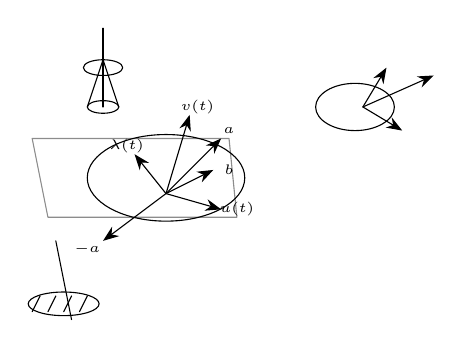
\begin{tikzpicture}[x=1mm,y=1mm,line cap=round,line join=round,font=\scriptsize]
\draw (21,-34) -- (21,-44);
\draw (19,-44) -- (21,-38) -- (23,-44);
\draw (21,-44) ellipse[x radius=2, y radius=0.8];
\draw[-{Stealth[length=2mm]}] (21,-39) ellipse[x radius=2.5, y radius=1];
\draw[pencil] (12,-48) -- (37,-48) -- (38,-58) -- (14,-58) -- cycle;
\draw (29,-53) ellipse[x radius=10, y radius=5.5];
\draw[-{Stealth[length=2mm]}] (29,-55) -- (36,-48);
\draw[-{Stealth[length=2mm]}] (29,-55) -- (35,-52);
\draw[-{Stealth[length=2mm]}] (29,-55) -- (21,-61);
\draw[-{Stealth[length=2mm]}] (29,-55) -- (36,-57);
\draw[-{Stealth[length=2mm]}] (29,-55) -- (32,-45);
\draw[-{Stealth[length=2mm]}] (29,-55) -- (25,-50);
\node[inner sep=1pt] at (37,-47) {\tiny $a$};
\node[inner sep=1pt] at (37,-52) {\tiny $b$};
\node[inner sep=1pt] at (19,-62) {\tiny $-a$};
\node[inner sep=1pt] at (38,-57) {\tiny $u(t)$};
\node[inner sep=1pt] at (33,-44) {\tiny $v(t)$};
\node[inner sep=1pt] at (24,-49) {\tiny $\lambda(t)$};
\draw (15,-61) -- (17,-71);
\draw (16,-69) ellipse[x radius=4.5, y radius=1.5];
\draw (12,-70) -- (13,-68);
\draw (14,-70) -- (15,-68);
\draw (16,-70) -- (17,-68);
\draw (18,-70) -- (19,-68);
\draw (53,-44) ellipse[x radius=5, y radius=3];
\draw[-{Stealth[length=2mm]}] (54,-44) -- (57,-39);
\draw[-{Stealth[length=2mm]}] (54,-44) -- (63,-40);
\draw[-{Stealth[length=2mm]}] (54,-44) -- (59,-47);
\end{tikzpicture}
\end{document}
